\documentclass[../../../main.tex]{subfiles}

\begin{document}
\setcounter{chapter}{11}
\chapter{Electrostatics}

\section{Coulomb's Law}

\begin{gather*}
    F=(\frac{1}{4\pi\epsilon_0})\frac{Q_1Q_2}{r^2}, \\
    \text{where } \epsilon_0= \text{permittivity of vacuum or free space}
\end{gather*}

\begin{mdframed}
    Definition: The magnitude of the electric force between two point charges is \emph{directly proportional to the product of the two charges} and \emph{inversely proportional to the square of the distance between them}.
\end{mdframed}
Given that F is inversely proportional to \(r^2\),
\begin{equation}
    F \propto \frac{1}{r^2}
\end{equation}
thus,
\begin{equation}
    \frac{F_1}{F_2}=(\frac{r_2}{r_1})^2
\end{equation}

\section{Electric Field}

\subsection{Electric Field}
\begin{mdframed}
    Definition: An electric field is a region in which an electric charge experiences a force. An electric field is represented by \textbf{electric field lines}.
\end{mdframed}

\pagebreak

\subsubsection{Electric Field Strength}
\begin{mdframed}
    Definition: The electric field strength at a point is the force per unit positive charge.
\end{mdframed}

The symbol for the electric field strength is \(E\) and it's unit is \(NC^{-1}\).
The direction of \(E\) at any point is the same as the direction of the force acting on a \textbf{positive test charge} placed at that point.

\begin{figure}[h]
    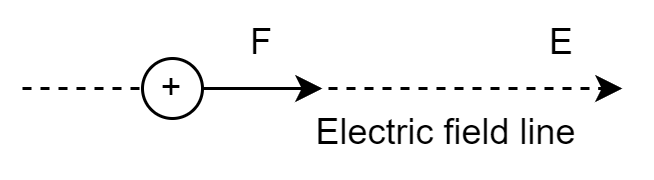
\includegraphics[scale=0.3]{figures/7.png}
    \centering
\end{figure}

If a charge Q is placed at a point which has an electric field intensity of E, then the force F acting on the charge is given by

\begin{equation}
    F=EQ
\end{equation}

\begin{figure}[h]
    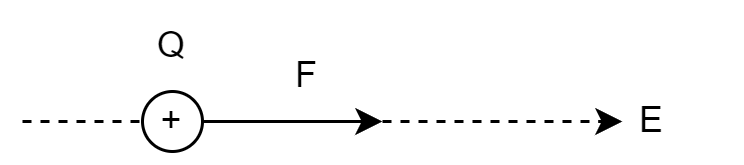
\includegraphics[scale=0.3]{figures/8.png}
    \centering
\end{figure}

\subsection{Electric Field by a Point Charge}

\subsubsection{Derivation of electric field strength formula at a point in an electric field produced by a point charge Q.}

\begin{figure}[h]
    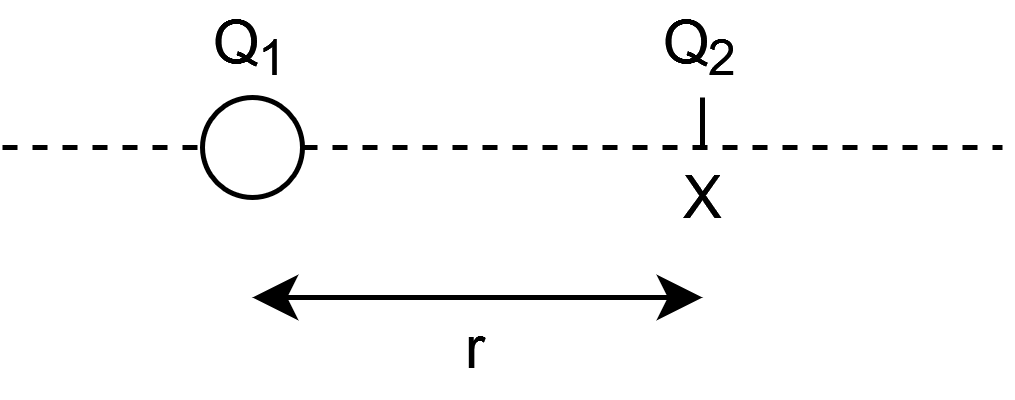
\includegraphics[scale=0.3]{figures/1.png}
    \centering
\end{figure}

\begin{align*}
    \text{Coulomb's Law: } F & =(\frac{1}{4\pi\epsilon_0})\frac{Q_1Q_2}{r^2}         \\
    F                        & =EQ_2                                                 \\
    E                        & =\frac{F}{Q_2}                                        \\
    E                        & =\frac{Q_1}{4\pi\epsilon_0r^2} \text{ (Substitute F)}
\end{align*}

\newpage

\subsubsection{Field Patterns}

\begin{figure}[h]
    \centering
    \subfloat[\centering Field pattern of a positive charge]{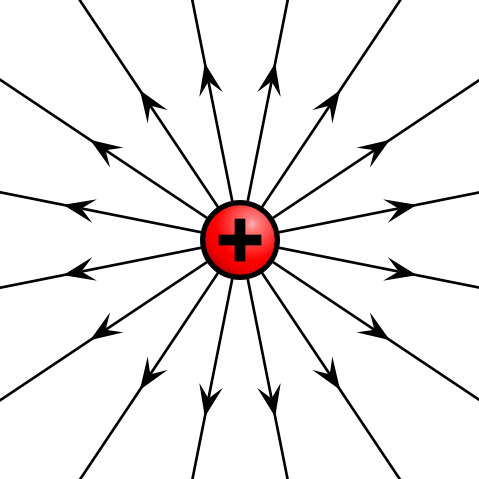
\includegraphics[scale=0.2]{figures/2.png}}
    \qquad
    \subfloat[\centering Field pattern of a negative charge]{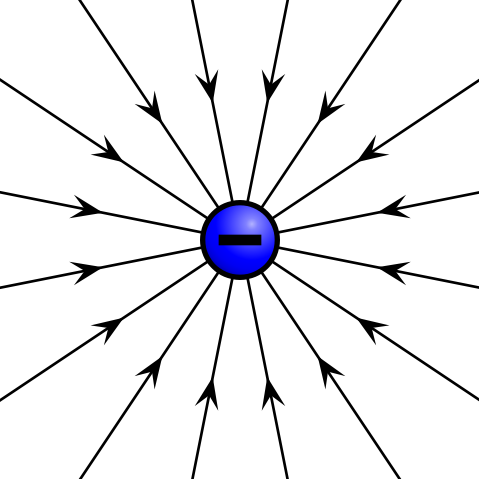
\includegraphics[scale=0.2]{figures/3.png}}
    \caption{Field patterns of charges}
\end{figure}

\begin{figure}[h]
    \centering
    \subfloat[\centering Field pattern of a dipole]{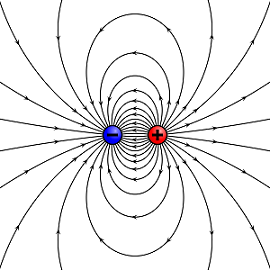
\includegraphics[scale=0.5]{figures/4.png}}
    \qquad
    \subfloat[\centering Field pattern of two positive point charges]{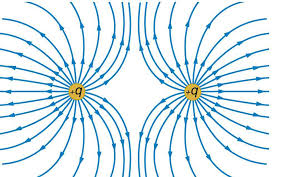
\includegraphics[scale=0.6]{figures/5.jpeg}}
    \caption{Field patterns of dipoles}
\end{figure}

\newpage

\subsection{Motion of a Charged Particle in a Uniform Electric Field}

\begin{figure}[h]
    \centering
    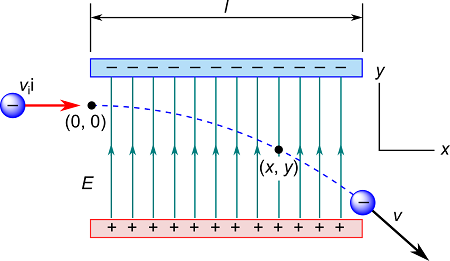
\includegraphics[scale=0.6]{figures/6.png}
\end{figure}

Horizontally, the charged particle's acceleration is zero, and moves at a constant velocity, \(u_x\).
\begin{gather*}
    \text{Horizontally, } \\
    a_x =0,               \\
    v_x =u_x,               \\
    \text{whereby \(u_x\) is the initial velocity.}
\end{gather*}

Vertically, it is acted on by an upward force \(EQ\), having a constant upward acceleration of $\frac{EQ}{m}$.
\begin{gather*}
    \text{Vertically,} \\
    F=EQ,             \\
    F=ma,             \\
    a=\frac{EQ}{m}
\end{gather*}

\newpage

\subsubsection{Commonly used formulae}
\begin{mdframed}
    Time spent inside the electric field:
    \begin{equation}
        t=\frac{L}{u_x}
    \end{equation}
\end{mdframed}

\begin{mdframed}
    Vertical displacement of the electron, \(h\):
    \begin{align}
        s                      & =ut+\frac{1}{2}at^2                           \\
        \text{Substituting } a & =\frac{EQ}{m} \text{ and } t=\frac{L}{u_x}    \\
        h                      & =0+\frac{1}{2}(\frac{EQ}{m})(\frac{L}{u_x})^2 \\
        h                      & =\frac{1}{2}(\frac{EQ}{m})(\frac{L}{u_x})^2
    \end{align}
\end{mdframed}

\begin{mdframed}
    Vertical velocity of the electron at B:
    \begin{align}
        v_y & =u_y+at                        \\
        v_y & =0+\frac{EQ}{m}(\frac{L}{u_x})
    \end{align}
\end{mdframed}

\begin{mdframed}
    Horizontal velocity of the electron at B:
    \begin{align}
        At \text{ B, } v_x & =u_x
    \end{align}
    \begin{center}
        (Since there is no horizontal acceleration, the horizontal velocity remains constant.)
    \end{center}
\end{mdframed}

\begin{mdframed}
    Actual velocity of the electron at B:
    \begin{align}
        v=\sqrt{v_x^2+v_y^2}
    \end{align}
\end{mdframed}

\begin{mdframed}
    Direction of the motion of the electron at B:
    \begin{align}
        \tan{\theta} & =\frac{v_y}{v_x}
    \end{align}
\end{mdframed}

\pagebreak

\begin{mdframed}
    Total linear deflection of the electron on the screen, \(GC=h+y\):
    \begin{align*}
        h  & = \frac{1}{2}(\frac{EQ}{m})(\frac{L}{u_x})^2,               \\
        y  & = D \tan{\theta}                                            \\
        GC & = \frac{1}{2}(\frac{EQ}{m})(\frac{L}{u_x})^2+D \tan{\theta}
    \end{align*}
    \begin{center}
        \(h=\) the \emph{parabolic} motion of the electron while in the electric field

        \(y=\) the \emph{linear} deflection of the electron after exiting the electric field
    \end{center}
\end{mdframed}

\newpage

\section{Gauss's Law}
\subsection{Gauss's Law}

\begin{gather*}
    \Phi=\frac{Q}{\epsilon} \\
    \text{where } \epsilon= \text{permittivity of the medium}
\end{gather*}

\begin{mdframed}
    Definition: The \textbf{net} electric flux, \(\Phi\), passing through a \textbf{closed surface} (Gaussian surface) is equal to the total net charge Q inside the closed surface divided by permittivity, \(\epsilon\), of the medium.
\end{mdframed}
If the charge is in vacuum, then Gauss's law is written as
\begin{gather*}
    \Phi=\frac{Q}{\epsilon_0} \\
    \text{where } \epsilon_0= \text{permittivity of vacuum}
\end{gather*}

\subsection{Application of Gauss Law}

\subsubsection{Using Gauss's Law to determine the electric field strength for an isolated point charge/charged spherical conductor:}
\begin{align*}
    \text{Gauss's Law: } \Phi & =\frac{Q}{\epsilon_0}        \\
    \intertext{\centering Because electric field intensity, \(E\) at a point can also be defined as the amount of electric flux per unit area (a.k.a. the electric flux density),}
    E                         & =\frac{\Phi}{A}              \\
    \intertext{\centering Substituting \(\Phi=\frac{Q}{\epsilon_0}\),}
    E                         & =\frac{Q}{\epsilon_0A}
    \intertext{\centering If the charge is uniformly distributed over the surface of a sphere with radius \(r\),}
    \text{Hence, } E          & =\frac{Q}{4\pi\epsilon_0r^2} \\
\end{align*}
\emph{This formula can also be applied for an isolated point charge.}

\bigskip

However, it must be noted that this formula is only applicable to situations in which the charge is \textbf{uniformly distributed at the surface of a sphere}.

\pagebreak

Inside the sphere, the electric field strength is zero, as the electric field lines cancel each other out.
\begin{equation*}
    \text{Hence}, E=0
\end{equation*}

Outside the sphere, at a distance of \(r\) from the center of the sphere, the electric field strength is given by
\begin{equation*}
    E=\frac{Q}{4\pi\epsilon_0r^2}\
\end{equation*}

\subsubsection{Using Gauss's Law to determine the electric field strength for a uniformly charged conducting plate:}

\begin{figure}[h]
    \centering
    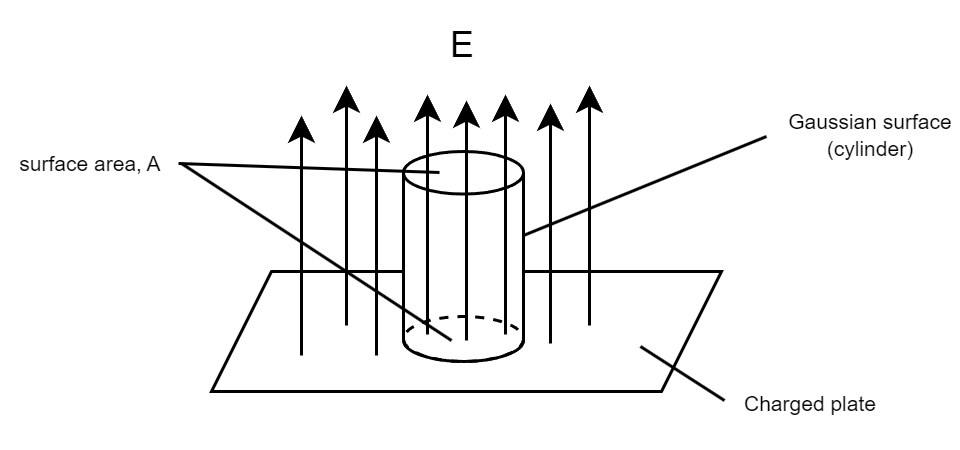
\includegraphics[scale=0.3]{figures/9.png}
\end{figure}

\begin{align*}
    \text{Gauss's Law: } \Phi & =\frac{Q}{\epsilon_0}      \\
    \intertext{\centering Because electric field intensity, \(E\) at a point can also be defined as the amount of electric flux per unit area (a.k.a. the electric flux density),}
    E                         & =\frac{\Phi}{A}            \\
    \intertext{\centering Substituting \(\Phi=\frac{Q}{\epsilon_0}\),}
    E                         & =\frac{Q}{\epsilon_0A}
    \intertext{\centering Assuming the charged plate (top surface of the cylinder) has a surface charge density of \(\sigma\) cm\(^{-2}\),}
    \sigma                    & =\frac{Q}{A}               \\
    Q                         & =\sigma A                  \\
    \text{Therefore, } E      & =\frac{\sigma}{\epsilon_0}
\end{align*}

\pagebreak

\section{Electric Potential}

\end{document}